\documentclass[]{revtex4}
\usepackage{graphicx}
\usepackage{amssymb}
\usepackage{epstopdf}
\usepackage{amsmath}
\usepackage{graphics}
\usepackage[mode = buildnew]{standalone}

\begin{document}

\title{Improving Laser Guide Stars through Magnetic Resonant Pulsing}

\author{M.K. and A.W.}
\affiliation{Willamette University}

\date{\today}

%%%%%%%%%%%%%%%%%%%%%%%%%%%%%%%%%%%%%%%%%%%%%%%%%%
% Abstract
%%%%%%%%%%%%%%%%%%%%%%%%%%%%%%%%%%%%%%%%%%%%%%%%%%

\begin{abstract}
%In this paper, we present the results on a method to increase the flurorescence of atoms confined in a magnetic field. The method, magnetic resonant pulsing, relies on pulsing a laser with circularly polarized light at the repetition rate of the Larmor frequency of the total atomic angular momentum vector of the atom. For atoms confined in a magnetic field oriented perpendicular to the laser beam, we show a 14\% increase in fluorescence when the repetition rate is in tune with the Larmor frequency. Furthermore, we show that the fluorescence of a laser in magnetic resonant pulsing decreases by only 2\% when the angle between the laser and magnetic field changes from $0^{\circ}$ to $90^{\circ}$, constrasted against a 34\% decrease with a continuous wave laser. This has applications to laser guide stars, which suffer from a degradation in brightness due to the Larmor precession of sodium atoms in the geomagnetic field.
Atoms with a magnetic moment residing in a magnetic field experience Larmor precession, a precession of the atom's total atomic angular momentum due to the torque the magnetic field exerts on the atom, with frequency known as the Larmor frequency. This precession degrades the benefits obtained through optical pumping, a technique used to increase atomic fluorescence, through a nonoptimal redistribution of the atom's angular momentum. However, according to Kane et al. (2014), a technique known as magnetic resonant pulsing suggests that laser light pulsed at the Larmor frequency can mitigate this degradation and increase atomic fluorescence by reestablishing the benefits of optical pumping. We test this technique by constructing a pulsed laser and measuring the fluorescence of rubidium confined in a magnetic field. We report a 32\% increase in fluorescence between CW and pulsed laser light when the laser beam is perpendicular to the magnetic field. This method can significantly increase the irradiance of laser guide stars due to the near-equatorial position of many telescopes, giving angles between their laser beams and the geomagnetic field of nearly $90 ^{\circ}$.



\end{abstract}


\maketitle

%%%%%%%%%%%%%%%%%%%%%%%%%%%%%%%%%%%%%%%%%%%%%%%%%%
% Introduction
%%%%%%%%%%%%%%%%%%%%%%%%%%%%%%%%%%%%%%%%%%%%%%%%%%
\section{Introduction}
Modern astronomy relies on the ability of telescopes to take high resolution images of distant celestial objects. However, due to atmospheric distortion, the quality of telescopic images taken from Earth is significantly reduced thereby limiting the ability of state-of-the-art ground based telescopes. In order to lessen the severity of atmospheric distortion, telescopes use two elements: an adaptive optics (AO) system and a laser guide star (LGS). The AO system, composed of a deformable mirror and a computer algorithm, records the image of the LGS, an artificial created by shining laser light into the atmosphere where it is absorbed and emitted by sodium atoms deposited by ablated meteors, then calculates the distortion the atmosphere imposes on the incoming light and subtracts this distortion from the image of the celestial object \cite{Wizinowich2006}. This significantly reduces the impact of atmospheric distortion.

In order for adaptive optics systems to perform well, they need to be able to collect as much information from the LGS as possible and, thus, a good LGS is very bright, ensuring that enough light is sent to the adaptive optics system. Therefore, LGS systems employ lasers of high intensity to achieve high irradiance. However, at higher intensities, the number of returned photons begins to decrease as laser intensity increases due to transition saturation (i.e. depumping), the decay of atoms to a lower ground state inaccessible to the specific wavelength of the laser. Thus, in addition to increasing laser intensity, many LGS systems use circularly polarized light to increase the number of returned photons through optical pumping. Using circularly polarized light establishes a cycling transition between the atom’s two highest angular momentum states, effectively creating a two level atomic system, which increases LGS brightness significantly. However, since sodium atoms possess a magnetic moment, they interact with the geomagnetic field of the Earth. The torque that this magnetic field exerts on the atom’s magnetic moment causes a precession of the atom’s total atomic angular momentum vector (Larmor precession) with a frequency known as the Larmor frequency (around 200-400 kHz in Earth’s magnetic field of around half of a Gauss). This precession decreases the overall efficiency of optical pumping since the atom’s angular momentum vector is changing in time, and a cycling transition between the atom’s two highest angular momentum states cannot be established. Thus, LGS are not achieving the highest irradiance possible, especially at latitudes near the equator where the angle between the laser beam and the direction of the magnetic field is greatest.

However, in a recent paper by Kane et al. \cite{Kane2014}, it is suggested that a method called magnetic resonant pulsing (MRP) can solve the issue of Larmor precession. MRP is the use of circularly polarized laser light pulsed specifically at the Larmor frequency of the atoms. This ensures that laser light is only interacting with the atoms at one point in their precession cycle, appearing as if the atom’s angular momentum vector is not changing in time with respect to the pulses of light. This allows a two-level cycling transition between the atom’s two highest angular momentum levels to be fully established, increasing the irradiance of LGS. We experimentally test MRP under controlled conditions determining that the fluorescence from MRP systems can be up to 30\% greater than fluorescence from continuous wave systems for telescopes near the equator.


\section{Theory}

One technique that is often used in LGS to increase atomic fluorescence is the use of circularly polarized laser light. Photons can carry spin angular momentum (SAM), and due to conservation of angular momentum, this momentum is imparted onto the atom upon absorption. When an atom absorbs a photon with SAM of $S_z = \pm \hbar$, the angular momentum of the atom must increase by the same amount, $\Delta m_J = \pm 1$. Then, upon emitting a photon, the atom can decay to any state satisfying $\Delta m_J = \pm 1, 0$. However, no matter which state the atom decays to, it will again be pumped back up with $\Delta m_j = +1$. Hence, atoms tend to move towards states of higher angular momentum and eventually end up in a cyclical transition between the states of highest angular momentum. This process, shown in Figure \ref{fig:opticalpumping}, is known as \textit{optical pumping} \cite{Kane2014}. By pumping all atoms into this two-level transition, we ensure that the atoms can only have one decay path with high probability, increasing photon emission and absorption by a factor of 3 \cite{Kibblewhite2009}.


\begin{figure}[ht]
	\centering
	\includestandalone{../FullPaper/Images/tikz/opticalpumping}
	\caption{Figure of optical pumping in which the excitation of the atom results in an angular momentum change of $\Delta m_j = +1$ but decay governed by $\Delta m_j = \pm 1, 0$ \protect\cite{opticalpumping}.}
	\label{fig:opticalpumping}
\end{figure}



However, when exposed to an external magnetic field, the $\vec J$ vector will tend to precess about the magnetic field, known as \textit{Larmor precession}. Classically, this precession can be thought of as due to the torque a magnetic field exerts on the atom,

\begin{equation}
  \vec \tau = \vec \mu \times \vec B,
  \label{larmortorque}
\end{equation}
%
where $\vec \mu$ is the magnetic moment of the atom and $\vec B$ is the external magnetic field. This equation can be rewritten by noting that the magnetic moment of the atom is the product of the gyromagnetic ratio and angular momentum of the atom,

\begin{equation}
  \vec \mu = \gamma \vec J,
  \label{magneticmoment}
\end{equation}
%
where $\vec J$ is the atom's combined angular momentum and $\gamma = g\frac{e}{2m}$ is the gyromagnetic ratio with $e$ being the charge of an electron, $g$ being the g-factor, and $m$ being the mass of the atom.
%
%\begin{equation}
%  \vec \tau = \gamma \vec J \times \vec B.
%  \label{larmortorque2}
%\end{equation}
%
The angular frequency of this precession, known as the \textit{Larmor frequency}, can be found by solving $\vec \tau = \frac{d\vec J}{dt}$, giving

\begin{equation}
  \omega = \gamma B.
  \label{larmorfrequency}
\end{equation}
%
From the Larmor frequency, we can compute the energy shift due to the magnetic field. This shift is
\begin{equation}
		\Delta E = \hbar \omega = \hbar \gamma B.
		\label{ehw}
\end{equation}
%
Larmor precession can actually degrade the benefits obtained by optical pumping. Optical pumping relies on redistributing the angular momentum of the atom, but for a magnetic field not aligned with the direction of the laser beam, this redistribution does not distribute angular momentum perfectly since the magnetic field reorients $\vec J$. Typically, the magnetic field reorients the atom much faster than the benefits of optical pumping can be obtained \cite{Kane2014}. Thus, the increase in absorption and emission is greatly reduced for atoms exposed to a magnetic field.


%Concerned with high luminosity 

%F is the total atomic angular momentum quantum number

However, if we substitute the energy shift from the Zeeman effect, given by Equation \ref{zeeman}, into Equation \ref{ehw}, we can find the frequency of the atom's precession,

\begin{equation}
	f_Z = \frac{\mu_B m_F g_F}{\hbar} B.
  \label{zeemanf}
\end{equation}
%
Instead of pumping the atoms continuously with light (using a CW laser), we can optically pump the atoms with light that is pulsed at a repetition rate equal to this frequency. This allows the light to only ``talk'' to the atoms at one point in the precession cycle, as if the particle were not precessing at all. The benefits of optical pumping can be reestablished with this technique, since a cycling transition can be reached without the combined angular momentum $\vec J$ changing in time. This technique is known as \textit{magnetic resonant pulsing}\footnote{The idea of magnetic resonant pulsing is analogous to pushing a child on a swing. If you apply a constant force the whole time, your child will not establish a nice oscillation. However, if you give a good push at one point each oscillation, your kid will soon be swinging quite high on the swing set.} \cite{Kane2014}.

%%%%%%%%%%%%%%%%%%%%%%%%%%%%%%%%%%%%%%%%%%%%%%%%%%
% discussion
%%%%%%%%%%%%%%%%%%%%%%%%%%%%%%%%%%%%%%%%%%%%%%%%%%
\section{Results}
The final experimental apparatus is shown schematically in Figure \ref{fig:expsetup} and actually in Figure \ref{fig:expsetupactual}. It consisted of the diode laser on resonance with the rubidium D2 line, capable of being pulsed or contiunuous wave, the main coils variable in strength and angle with respect to the laser beam, compensation coils to rid the geomagnetic field, the rubidium cell, and two photodiodes to measure fluorescence from the top of the cell (photodiode 1) and to measure backscatter (photodiode 2). 

\begin{figure}[ht]
	\centering
	\includestandalone[width = .9\textwidth]{../FullPaper/Images/tikz/fluorescence}
	\caption{Schematic of the experimental setup to measure fluorescence of rubidium atoms including the Helmholtz coils, rubidium cell, and photodiode.}
	\label{fig:expsetup}
\end{figure}

\begin{figure}[htpb]
	\centering
	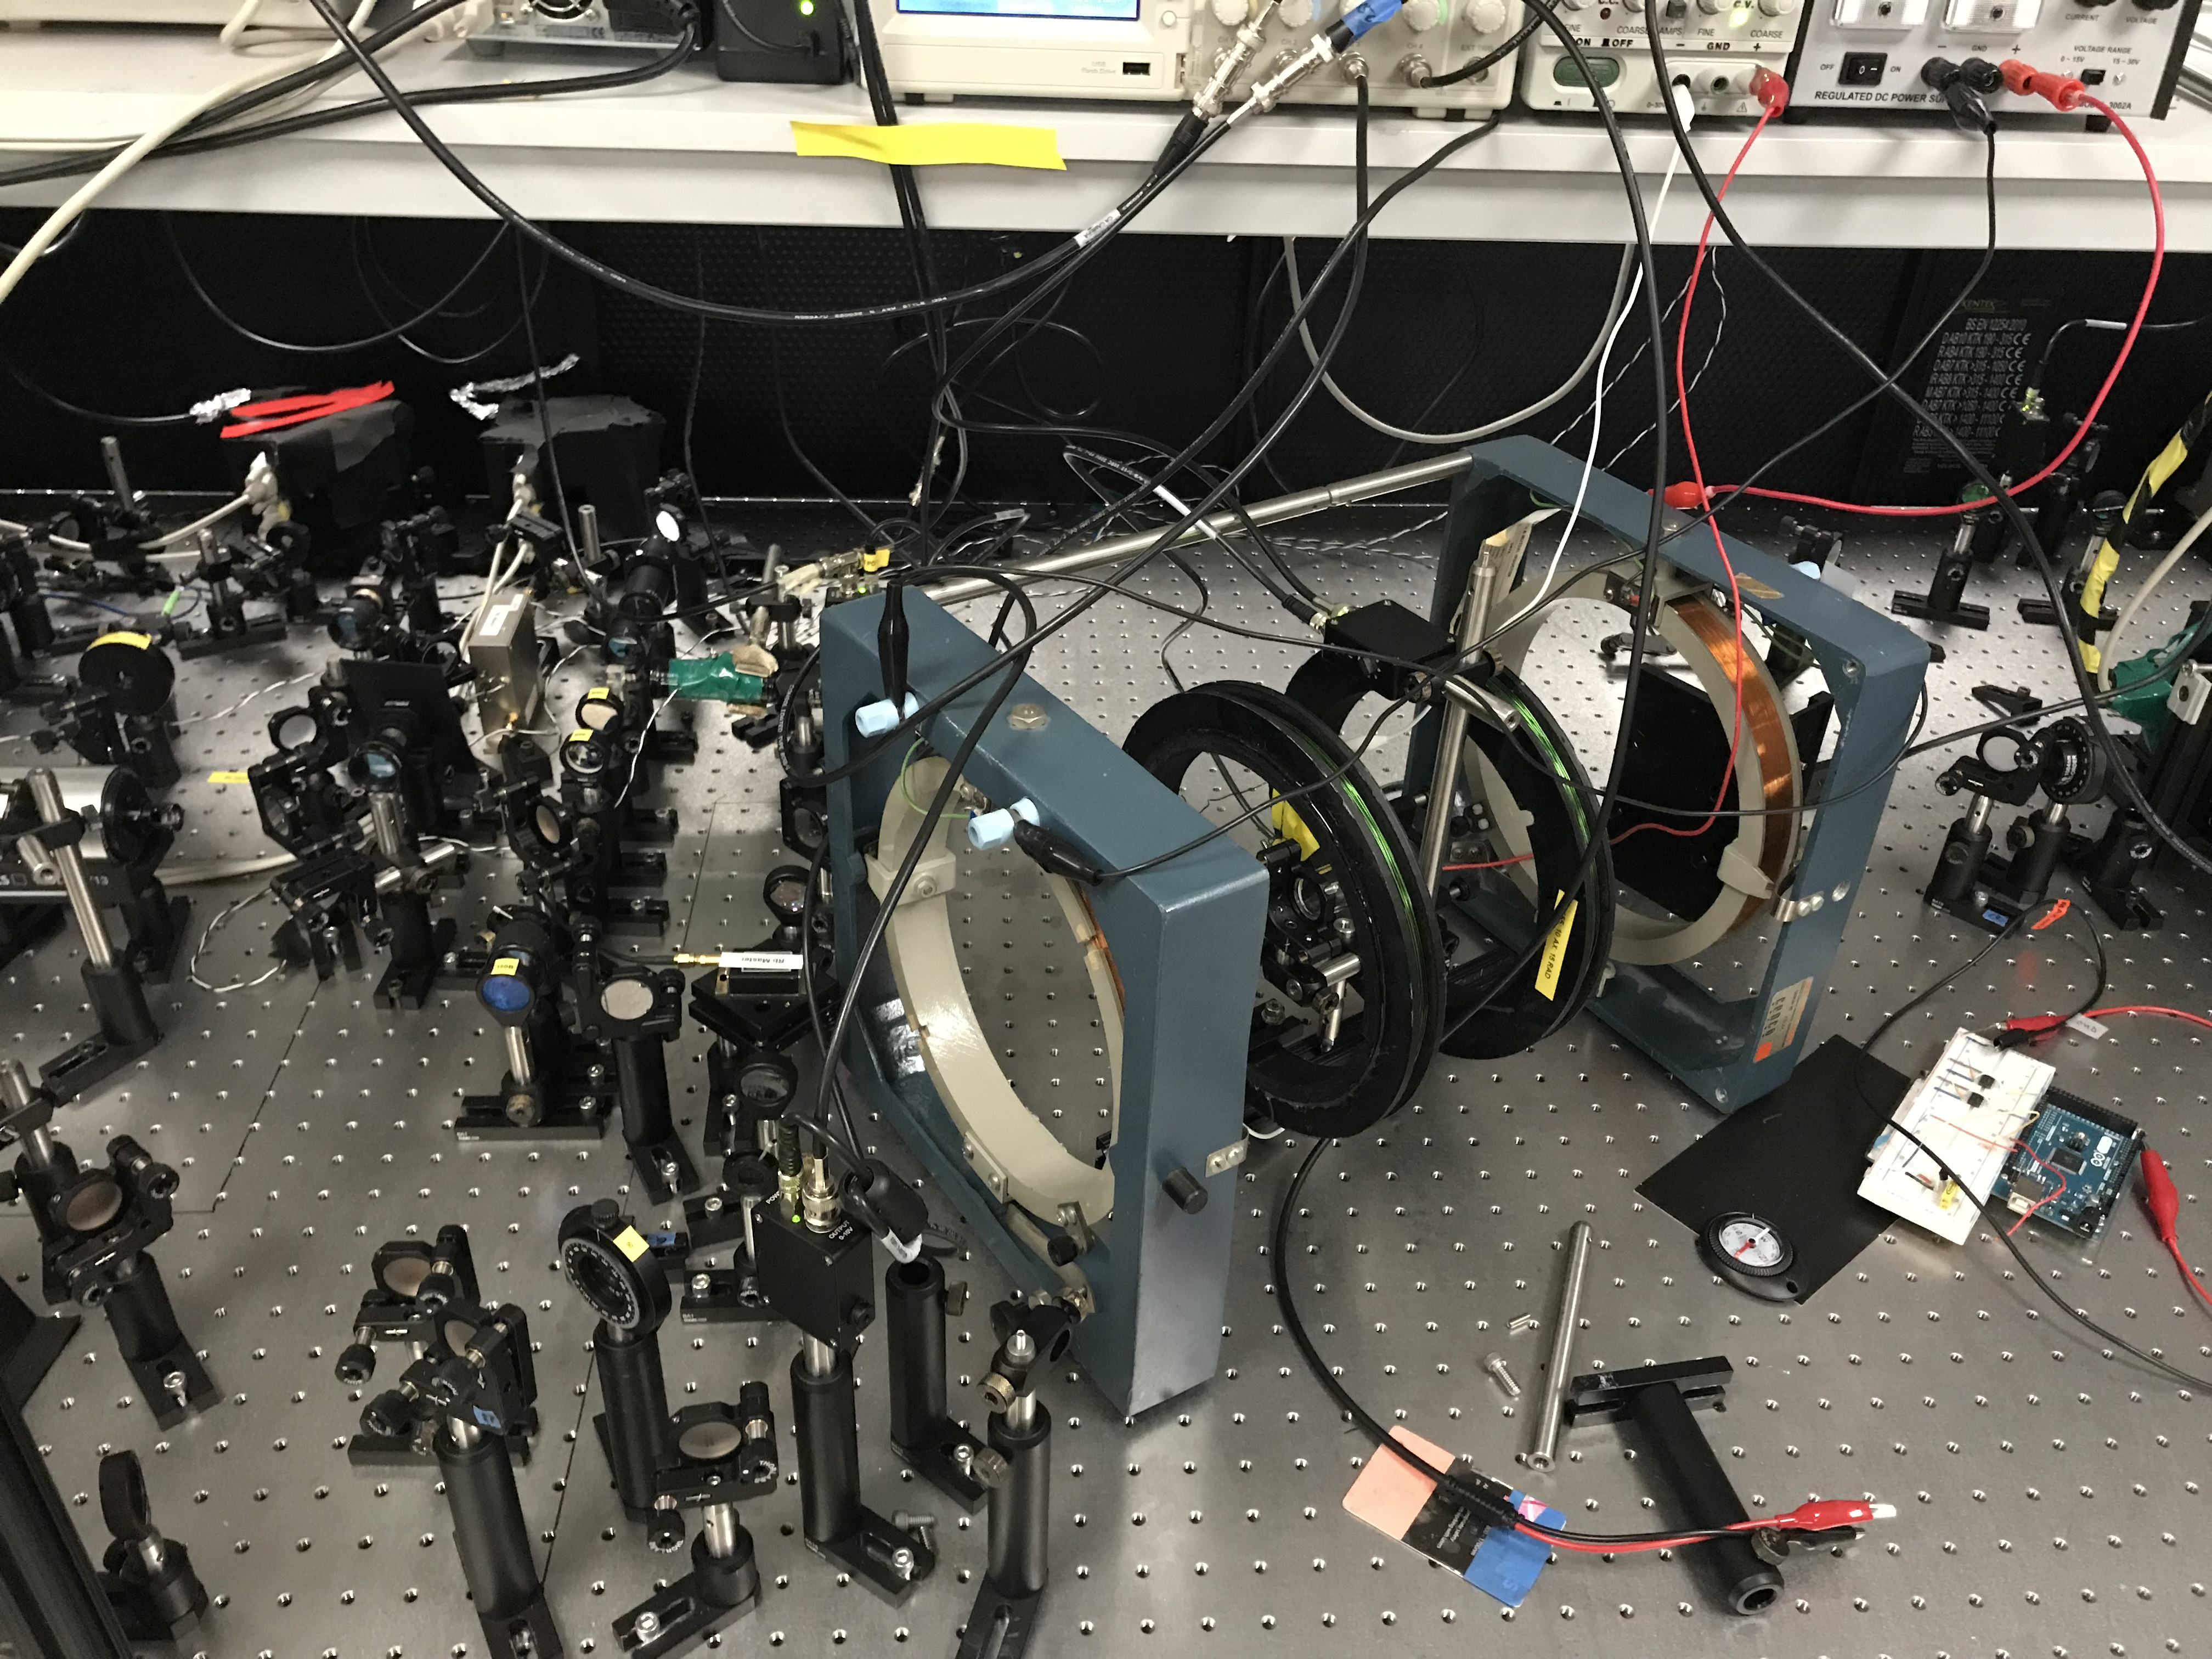
\includegraphics[width=0.8\textwidth]{../FullPaper/Images/setup.png}
	\caption{Experimental setup shown with compensation coils, main coils, absorption cell, and laser beam.}
	\label{fig:expsetupactual}
\end{figure}

The first measurement taken was a confirmation of the validity of magnetic resonant pulsing. An arbitrary current was chosen (0.12 A), from this the magnetic field was calculated using Equation \ref{eq:fieldvcurrent}, and then the Larmor frequency of rubidium was calculated using Equation \ref{zeemanf}, repeated below with numerical factors substituted in:

\begin{equation}
	\begin{split}
		f & = \frac{\mu_B g_f m_f}{h} \text{B}\\
		  & \approx 0.47 \text{ B Mhz}.
\end{split}
	\label{eq:larmorvB}
\end{equation}
%
The repetition rate of the diode laser was set to this Larmor frequency, and the magnetic field was set perpendicular to the laser beam. From here, current was varied around the 0.12 A, changing the magnetic field. The expected result was an increase in the fluorescence around 0.12 A. This increase in fluorescence was found, and is shown in Figure \ref{fig:flvc}. The fluorescence was measured by reading the a change in intensity (in volts) on an oscilloscope, and dividing this value by the average power of the diode laser.


\begin{figure}[htpb]
	\centering
	\includegraphics[width=0.8\textwidth]{../FullPaper/../../MRPData/EfficiencyCurr.pdf}
	\caption{Fluorescence versus current with magnetic field perpendicular to laser beam and the repetition rate set at \SI{700}{ kHz}. The expected increase at 0.12 A is seen.}
	\label{fig:flvc}
\end{figure}

The second measurement taken was of fluorescence versus repetition rate with a constant magnetic field (of a few gauss) perpendicular to the laser beam. With the current set to 0.12 A, the expected peak in fluorescence would peak at \SI{700}{ kHz}. This was found to be true and is shown in Figure \ref{fig:flvrep}.

This confirmed that MRP indeed increases the fluorescence of atoms. We report a 14\% increase in fluorescence at the Larmor frequency repetition rate, with a bandwidth of approximately \SI{50}{ kHz}.

\begin{figure}[ht]
	\centering
	\includegraphics[width=0.8\textwidth]{../FullPaper/../../MRPData/MAR24/FLvRep.pdf}
	\caption{Fluorescence of rubidium in a magnetic field of approximately a few Gauss perpendicular to laser beam as a function of repetition rate. The peak at \SI{700}{ kHz} shows the increase in fluorescence at the Larmor frequency of the atoms.}
	\label{fig:flvrep}
\end{figure}


The final measurement taken was of the fluorescence versus the angle between the magnetic field and the laser beam. The magnetic field was tuned to the repetition rate such that the system was in MRP and there was a maximum in fluorescence. Fluorescence measurement were then taken with respect to changes in the angle of the magnetic field. The expected result was a constant fluorescence for all magnetic field angles. Data was also taken with a continuous wave laser. The expected result was a decrease in fluorescence with increasing magnetic field angle. Both of these expected results were confirmed and are shown in Figure \ref{fig:flvangle}. These measurements were also taken with linearly polarized light in order to confirm that our results were truly from magnetic resonant pulsing. The results were consistent with the theory of MRP.



\begin{figure}[ht]
	\centering
	\includegraphics[width=0.8\textwidth]{../../MRPData/MAR24/together.pdf}
	\caption{Fluorescence of rubidium atoms in a magnetic field of approximately a few Gauss as a function of the angle between the field and the laser beam. Data of pulsed and continuous laser light circularly and linearly polarized are shown. Circularly polarized light with a repetition rate equal to the Larmor frequency gives the highest return for all magnetic field orientations.}
	\label{fig:flvangle}
\end{figure}

To visulaize changes in fluorescence with angle, we calculate the percent changes from maximum fluorescence, and plot them as well. These data are shown in Figure \ref{fig:flvanglescaled}. We report a 33\% decrease in fluorescence for continuous wave, circularly polarized laser beams and a 2\% decrease in fluorescence for MRP laser beams at an angle of $90 \degrees$ between the laser beam and the magnetic field..

\begin{figure}[ht]
	\centering
	\includegraphics[width=0.8\textwidth]{../../MRPData/MAR24/togetherscaled.pdf}
	\caption{Percent changes fluorescence with respect to the maximum of rubidium atoms in a magnetic field of approximately a few Gauss as a function of the angle between the field and the laser beam. Data of pulsed and continuous laser light circularly and linearly polarized are shown. Circularly polarized light with a repetition rate equal to the Larmor frequency gives the highest return for all magnetic field orientations.}
	\label{fig:flvanglescaled}
\end{figure}



The previous data was measured using photodiode 1 (from top down). In order to  ensure that backscatter fluorescence indeed followed these same trends, we took two data points, at $0 \degrees$ and $90$ \degrees measured with photodiode 2 (backscatter). The data confirms that it behaves similarly and the expected results were obtained and are shown in Figure \ref{fig:backscatter} and scaled as percent changes in maximum fluorescence in Figure \ref{fig:backscatterscaled}.

\begin{figure}[ht]
	\centering
	\includegraphics[width=0.8\textwidth]{../../MRPData/Backscatter/backscatter.pdf}
	\caption{Fluorescence from maximum fluorescence for circularly polarized light with continuous light and light with repetition rate equal to that of the Larmor frequency. It is seen that backscatter agrees well with the data taken from top down.}
	\label{fig:backscatter}
\end{figure}

\begin{figure}[ht]
	\centering
	\includegraphics[width=0.8\textwidth]{../../MRPData/Backscatter/backscatterScaled.pdf}
	\caption{Change in backscatter fluorescence from maximum fluorescence for circularly polarized light with continuous light and light with repetition rate equal to that of the Larmor frequency. It is seen that backscatter agrees well with the data taken from top down.}
	\label{fig:backscatterscaled}
\end{figure}


%%%%%%%%%%%%%%%%%%%%%%%%%%%%%%%%%%%%%%%%%%%%%%%%%%
% Bibliography
%%%%%%%%%%%%%%%%%%%%%%%%%%%%%%%%%%%%%%%%%%%%%%%%%%
\bibliographystyle{alpha}
\bibliography{thesisbib}

\end{document}

